\documentclass[nogrid]{MBE}%

\usepackage{url}

\jshort{mst}

\volname{}

\jvolume{0}

\jvol{}

\jissue{0}

\pubyear{2019}

\mstype{Article}

\artid{012}

\begin{document}

\title{Tempo and mode of promoter evolution as observed in the \textit{Paramecium aurelia} species complex}

\author[Raborn et al.]{R. Taylor \surname{Raborn},$^{\ast,1,2}$ Timothy Licknack,$^{1,2}$ Shannon N. Snyder,$^{1,2}$ Tia Swenty,$^{1,2}$ Wanfeng Guo,$^{1,2}$ and Michael Lynch$^{1,2}$}

\address{$^{1}$Biodesign Institute Center for the Mechanisms of Evolution\\
$^{2}$School of Life Sciences\\
Arizona State University, 797 E. Tyler Street, Tempe, AZ 85281}


%\history{Received xx xxxxx 2020; reviews returned xx xxxx 2020; accepted xx xxxxx 2020}

\coresp{E-mail: rtraborn@asu.edu}

\abstract{Goes here}

\keyword{\textit{cis}-regulatory regions, duplicate genes, paralogous genes, \textit{Paramecium}, promoter evolution, TSS profiling.}


\maketitle


\section{{Introduction}\label{sec:Intro}}

A major challenge in genomics is to decipher the precise instructions that regulate gene expression. Differences in gene regulatory regions regions has long been posited to underlie a large part of the diversification seen across species (xxxx King and Wilson, 1975), and indeed investigations across select eukaryotes have drawn attention to the contributions of \textit{cis}-regulatory sequences in the evolution of gene expression differences \citep{Wittkopp:2008ki, Wittkopp:2011bc, Siepel:2014hd}. Work over the previous two decades have emphasized the contribution of \textit{cis}-regulatory sequence differences toward changes in gene expression \citep{Wittkopp:2004cy}. The fulcrum and first major step of gene expression is transcription initiation, which in eukaryotes begins with the mediated interaction of RNA polymerase II complex with the promoter, a \textit{cis}-regulatory region located proximal to the gene \citep{Kadonaga:2011gz}. The locations of eukaryotic \textit{cis}-regulatory sequences, including promoters, cannot be predicted from genome sequence alone with precision.\\

Comparative and functional genomic approaches have shed light on the contributions of \textit{cis}-regulatory sequences to phenotypic evolution and species divergence. Investigating F1 hybrids of \textit{D. melanogaster} and \textit{D. simulans}, Wittkopp and colleagues \citep{Wittkopp:2004cy} showed that interspecific expression differences were primarily caused by changes acting in \textit{cis}, not \textit{trans}. Evolutionary changes in gene expression patterns have been noted in a number of instances, including in expression timing (\textit{i.e.} heterochrony) \citep{Wray:1989ku}, expression levels (\citep{Crawford:1999ic}), spatial differences \citep{Abzhanov:2000vb}, and sex-specific expression \citep{Kopp:2000bl}; reviewed in \citep{Wray:2003kn}. The structure and conservation of the regulatory regions of select genes, including the \textit{hox} \citep{Kmita:2002hg} and \textit{pax} \citep{Plaza:1999kc} gene complexes, were established. More recently, the advent of large-scale functional genomics methods has identified sequence variants within regulatory regions that contribute to expression differences \citep{Lappalainen:2013el,Pickrell:2010bq, Schor:2017fw}; a number of these have been functionally characterized. Global functional genomics efforts have revealed the cellular mechanisms of transcriptome and regulatory variation, but have largely been confined to major model systems, especially human, and have not focused on exploring the changes to \textit{cis}-regulatory regions over evolutionary time-scales. As it stands, the precise \textit{cis}-regulatory sequence differences that accompany---or indeed underpin---species divergence remain largely obscure. Another potential explanation for this is the difficulty in predicting \textit{cis}-regulatory regions from genomic sequence alone. As such, accurate estimation of promoter positions requires direct, experimental evidence. At present, the most efficient approach to identify promoters at genome-scale is transcription start site (TSS) profiling, which includes CAGE (Cap Analysis of Gene Expression) \citep{Murata:2014gpb} and RAMPAGE \citep{Batut:2013fu}, among others. While TSS profiling methods differ in technical between themselves, these protocols all capture the 5$`$-ends of capped mRNAs, sequence their corresponding cDNAs and align the reads to the genome to identify the TSSs present within a given transcriptome. Clustering gene-adjacent TSSs defines a promoter, transcription start region (TSR), at single base-pair resolution, thereby providing genomic locations for \textit{cis}-regulatory regions within a species \citep{Lenhard:2012ena,Rach:2009ct}. TSS profling studies in a variety of model organisms has demonstrated that the shape of TSS distributions (\textit{i.e.} promoter shape) at promoters is related to the promoter class and correlates with the function of the associated gene \citep{Carninci:2006in, Rach:2009ct,Hoskins:2011io,Raborn:2016cr}. In addition, recent work done in \textit{Drosophila melanogaster} provides evidence that promoter shape is itself a quantitative trait \citep{Schor:2017fw}, a finding that carries valuable implications for the understanding of the evolution of \textit{cis}-regulatory regions. \\

A limited number of studies have investigated the evolution of promoters using TSS profiling information. Frith \textit{et al}. \citep{Frith:2006bb} compared TSSs between human and mouse tissues using the first generation of CAGE data. The authors observed ~1250 instances of shifting promoter usage within homologous sites, as well as tissue-specific TSS differences between species. Frith and colleagues also found that, consistent with expectations, TSSs with high turnover exhibited less sequence conservation in its promoter region than those without. The authors propose a model of gradual shifting between TSSs via alternative initiation sites, as well as shifting of initiation along the sequence itself. \\

Main et al. \citep{Main:2013dg}, used a separate TSS profiling method in \textit{D. melanogaster} to identify putative orthologous TSSs in three other \textit{Drosophila} taxa: \textit{D. simulans}, \textit{D. pseudoobscura} and \textit{D. sechellia}. The authors found that the location and estimated activities of orthologous TSSs to be generally conserved, but did observe instances of TSS variation indicative of new promoters. Notably, Main \textit{et. al.} found differences in promoter selection in the Alcohol dehydrogenase (ADH) gene across the four \textit{Drosophila} species \citep{Main:2013dg}. Working with high-resolution promoter data in human and mouse, Young and colleagues \citep{Young:2015xx} found that more than half (56\$) of tissue-matched promoters were lost, or turned over, between the two species. Noting that most protein-coding genes in mammals \citep{FANTOMConsortiumandtheRIKENPMIandCLSTDGT:2014hz} have multiple promoters, the authors propose that promoter turnover is an important but overlooked means by which transcriptional modules diverge during evolution. Li and colleagues (2018) investigated the fates of TSSs across  the primate lineage. They found that new TSSs frequently emerge in transposable elements and repetitive regions of DNA, and are more likely to emerge in areas near existing regulatory regions. While this work was valuable, demonstrating potential routes of regulatory innovation, the study was limited by the fact it only used empirically-defined TSSs in human (as those from other primates were not available), a fact that prevented the study from identifying novel promoters in the other primate taxa in the study. // 

Duplicate genes are a major source of evolutionary change (cite \citep{Ohno:1970wm} Moore and Puruggnan, 2006), and their evolutionary fates have long been a subject of intense study (reviewed in  The availability of high-quality genome assemblies and genome annotations has allowed us to investigate duplicate gene evolution in a variety of phylogenetic contexts (cite Gu et al., 2003 and others). However, while the fates of ortho-paralog pairs that arise through whole genome duplication (WGD) has been heavily studied (enter citations for \citep{Ohno:1970wm}; Wolfe and Shields, 1997, Force et al., 1999, others), the fates of \textit{cis}-regulatory regions of duplicate gene pairs is much less well-understood. (Discuss Haberer et al., Dong et al and Arsovski et al). 

(Add a bit about paralogs and how we can use them to help us understand how \textit{cis}-regulatory regions evolve. then:
-Add a paragraph introducing the Paramecium system -> the experiment\\
-Final sentence(s) of intro: what we found plus the novelty eg this is the first study of its kind to do x.

\section{Demographic structure}

Lorem ipsum dolor sit amet, consectetur adipiscing elit, sed do eiusmod tempor incididunt ut labore et dolore magna aliqua. Ut enim ad minim veniam, quis nostrud exercitation ullamco laboris nisi ut aliquip ex ea commodo consequat. Duis aute irure dolor in reprehenderit in voluptate velit esse cillum dolore eu fugiat nulla pariatur. Excepteur sint occaecat cupidatat non proident, sunt in culpa qui officia deserunt mollit anim id est laborum.

\subsection{Subsection 1}

Lorem ipsum dolor sit amet, consectetur adipiscing elit, sed do eiusmod tempor incididunt ut labore et dolore magna aliqua. Ut enim ad minim veniam, quis nostrud exercitation ullamco laboris nisi ut aliquip ex ea commodo consequat. Duis aute irure dolor in reprehenderit in voluptate velit esse cillum dolore eu fugiat nulla pariatur. Excepteur sint occaecat cupidatat non proident, sunt in culpa qui officia deserunt mollit anim id est laborum.


\subsubsection{Subsection 2}

Lorem ipsum dolor sit amet, consectetur adipiscing elit, sed do eiusmod tempor incididunt ut labore et dolore magna aliqua. Ut enim ad minim veniam, quis nostrud exercitation ullamco laboris nisi ut aliquip ex ea commodo consequat. Duis aute irure dolor in reprehenderit in voluptate velit esse cillum dolore eu fugiat nulla pariatur. Excepteur sint occaecat cupidatat non proident, sunt in culpa qui officia deserunt mollit anim id est laborum.


\paragraph{Paragraph header} 

Lorem ipsum dolor sit amet, consectetur adipiscing elit, sed do eiusmod tempor incididunt ut labore et dolore magna aliqua. Ut enim ad minim veniam, quis nostrud exercitation ullamco laboris nisi ut aliquip ex ea commodo consequat. Duis aute irure dolor in reprehenderit in voluptate velit esse cillum dolore eu fugiat nulla pariatur. Excepteur sint occaecat cupidatat non proident, sunt in culpa qui officia deserunt mollit anim id est laborum.

\section{{Methods}\label{sec:Methods}}

Lorem ipsum dolor sit amet, consectetur adipiscing elit, sed do eiusmod tempor incididunt ut labore et dolore magna aliqua. Ut enim ad minim veniam, quis nostrud exercitation ullamco laboris nisi ut aliquip ex ea commodo consequat. Duis aute irure dolor in reprehenderit in voluptate velit esse cillum dolore eu fugiat nulla pariatur. Excepteur sint occaecat cupidatat non proident, sunt in culpa qui officia deserunt mollit anim id est laborum.

\section{{Results}\label{sec:Results}}

Lorem ipsum dolor sit amet, consectetur adipiscing elit, sed do eiusmod tempor incididunt ut labore et dolore magna aliqua. Ut enim ad minim veniam, quis nostrud exercitation ullamco laboris nisi ut aliquip ex ea commodo consequat. Duis aute irure dolor in reprehenderit in voluptate velit esse cillum dolore eu fugiat nulla pariatur. Excepteur sint occaecat cupidatat non proident, sunt in culpa qui officia deserunt mollit anim id est laborum.

\section{{Discussion}\label{sec:Discussion}}

Lorem ipsum dolor sit amet, consectetur adipiscing elit, sed do eiusmod tempor incididunt ut labore et dolore magna aliqua. Ut enim ad minim veniam, quis nostrud exercitation ullamco laboris nisi ut aliquip ex ea commodo consequat. Duis aute irure dolor in reprehenderit in voluptate velit esse cillum dolore eu fugiat nulla pariatur. Excepteur sint occaecat cupidatat non proident, sunt in culpa qui officia deserunt mollit anim id est laborum.

\begin{arabiclist}
\item Item 1

\item Item 2

\item Item 3
\end{arabiclist}

\begin{itemize}
\item Consider a fall in population induced by a decline in the number of births in the economy,
taking as given mortality and migration.

\item It is well known that a lower population growth raises the capital--labor ratio in the Solow--Swan
growth model.

\item The same property holds in Diamond's (1965) overlapping generations model, and it enhances welfare
as long as the economy is dynamically efficient; i.e., when the interest rate exceeds the
population growth rate.
\end{itemize}
 A similar trend is observed in the United
States and advanced European countries (Gustafsson and Kalwij, 2006), and also in Canada,
Australia, and New Zealand (Sardon, 2006). Interestingly, as pointed out by Bongaarts and Feeney
(1998), even when the cohort's lifetime fertility rate (the number of children a mother has in her
lifetime) does not fall, the delayed childbearing alone leads to a decline in the number of
childbirths, measured by the total period fertility rates (TPFRs). %Ogawa and Retherford (1993),
%Kohler et al. (2002), and Sobotka (2004) confirmed that, to a certain extent, the delay of
%marriage and motherhood is responsible for the observed period fertility rate decline (now known
%as the `tempo effect').


\section{Model\label{sec:Model}}

\subsection{Demographic structure}



i.e.:
\begin{equation}
\lambda_{t}=\left\{
\begin{array}
[c]{cc}%
0, & t<0,\\
\lambda, & t\geq0.
\end{array}
\right.  \label{eq:lambda}%
\end{equation}


\begin{figure}[t]
\begin{center}
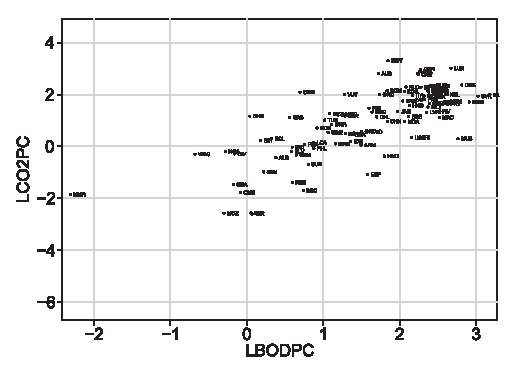
\includegraphics[height=0.21\textheight]{flrf1.eps}
\end{center}
\caption{Fluctuations in Cohort Size $N_{t}$ over Generations.}%
\label{fig:popdynamics}%
\end{figure}

%\TWOfig{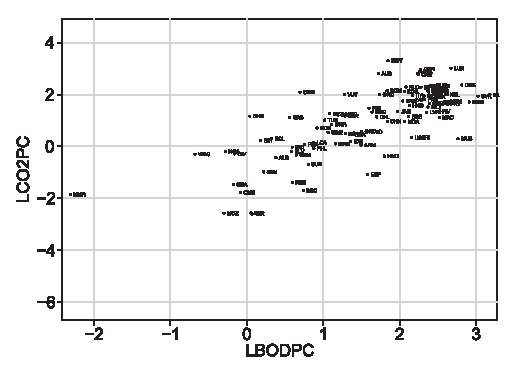
\includegraphics[width=10pc]{flrf1.eps}}{Fluctuations in
%Cohort Size $N_{t}$ over
%Generations.\label{fig:popdynamics}}{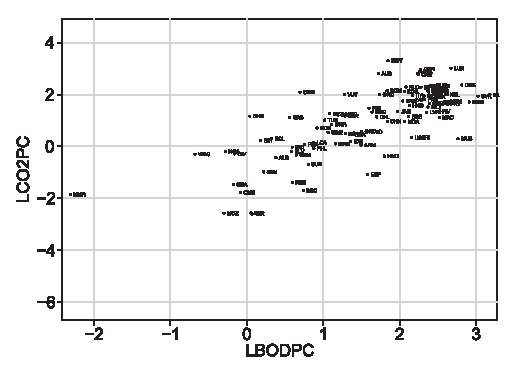
\includegraphics[width=10pc]{flrf1.eps}}{Dynamics
%of Labor Force $L_{t}$.\newline
%\phantom{\hskip5pc}\label{fig:labordynamics}}

where $C$ is a constant term defined as $C\equiv\beta\log\beta-(1+\beta
)\log(1+\beta)+\beta\log A\alpha+(1+\beta)\log A\left(  1-\alpha\right)  $.
Similarly, long-term welfare in the benchmark economy ($\lambda=0$) can be
written as:
\begin{equation}
U^{\ast}=\left(  1+\beta\right)  \log[A\alpha\left(  k^{\ast}\right)
^{2\alpha-1}+\left(  k^{\ast}\right)  ^{\alpha}]-\beta\left(  1-\alpha\right)
\log k^{\ast}+C. \label{eq:U_benchmark}%
\end{equation}

\begin{table}[!t]%1
\tableparts{\caption{SH test results on nuclear and mitochondrial phylogenetic trees}\label{tab1}}
{\begin{tabular*}{\columnwidth}{@{\extracolsep{\fill}}lld{6,0}d{6,0}@{}}\toprule Sequence data &
\mcc{Tree} & \mcc{$-\ln~L$} & \mcc{SH test $P$-value} \\\colrule mtDNA& mtDNA& -109219.5& 0.5 \\
[0.1pt]
mtDNA& Nuclear& -61720.8& \mcc{\hspace*{5pt}$<{0.00001}$} \\
Nuclear& mtDNA& -113033.1& \mcc{\hspace*{5pt}$<{0.00001}$} \\
Nuclear& Nuclear& -60699.9& 0.5 \\\botrule
\end{tabular*}}
{}
\end{table}

%
\section{Supplementary Material}
Supplementary tables S1?S7 and figures S1?S11 are available  at Molecular Biology and Evolution
online (http://www.mbe.oxfordjournals.org/).

\section{Acknowledgments}

The authors gratefully acknowledge the help of Robert Policastro and Gabriel Zentner at Indiana University Bloomington for technical assistance and use of laboratory facilities.


\bibliographystyle{natbib}%%%%natbib.sty
\bibliography{refs}%%%refs.bib

\end{document}
